\subsection{Quantum óptimo del SchedRR}

Para determinar el $quantum$ óptimo del scheduler $Round$ $Robin$ simulamos un lote de tareas $TaskBach$ utilizando el algoritmo SchedRR teniendo en cuenta las métricas mencionadas anteriormente: waiting time y turnaround time. Diseñamos el lote de la siguiente manera:
\begin{itemize}
	\item Cantidad de tareas: 30. Nos pareció un número adecuado para llevar a cabo el experimento.
	\item Uso de Cpu: igual para todas, 30.
	\item Cantidad de bloqueos: variados, entre 1 y 30.
\end{itemize}
(El lote de tareas utilizado puede encontrarse en el archivo $loteBatch.tsk$.)

Los costos de cambio de contexto y migración se fijaron en 1 y 2 (ciclos) respectivamente. Experimentamos utilizando varios núcleos de procesamiento.
Graficamos los resultados de waiting time y turnaround time en función del quantum seteado para 2,3 y 4 cores. Debido a que las tareas $TaskBatch$ realizan bloqueos en momentos elegidos pseudoaleatoriamente nos pareció correcto que, para un quantum dado, se obtengan varias veces (unas veinte) el waiting time y turnaround time para luego calcular un promedio. A su vez, tuvimos en cuenta el desvío estandar para realizar las barras de error en los gráficos. Los resultados obtenidos fueron los siguientes:

\begin{figure}[H]
	\begin{center}
		  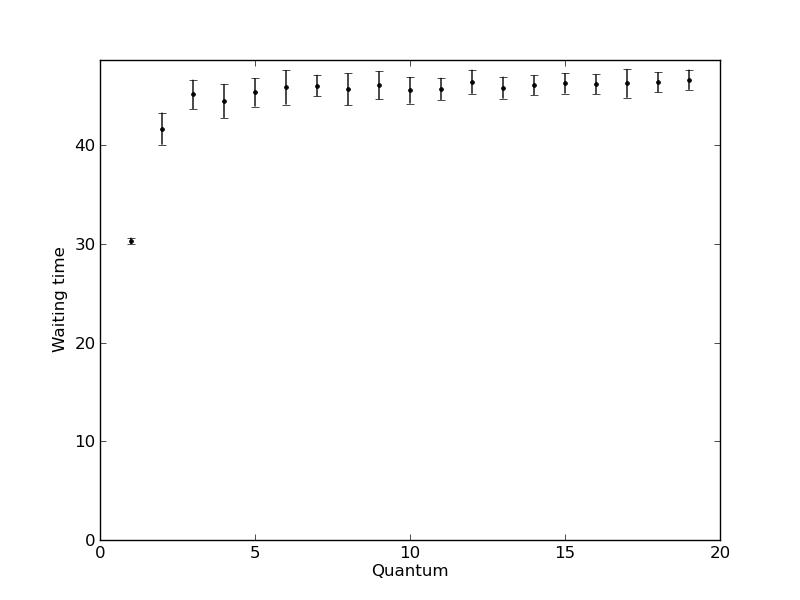
\includegraphics[scale=0.3]{graficos/cores_2_wt.jpg}
		  \caption{Gráfico de Waiting time en función del quantum con 2 cores para lote de tareas $taskBatch$}
		  \label{fig:contra1}
	\end{center}
\end{figure}

\begin{figure}[H]
	\begin{center}
		  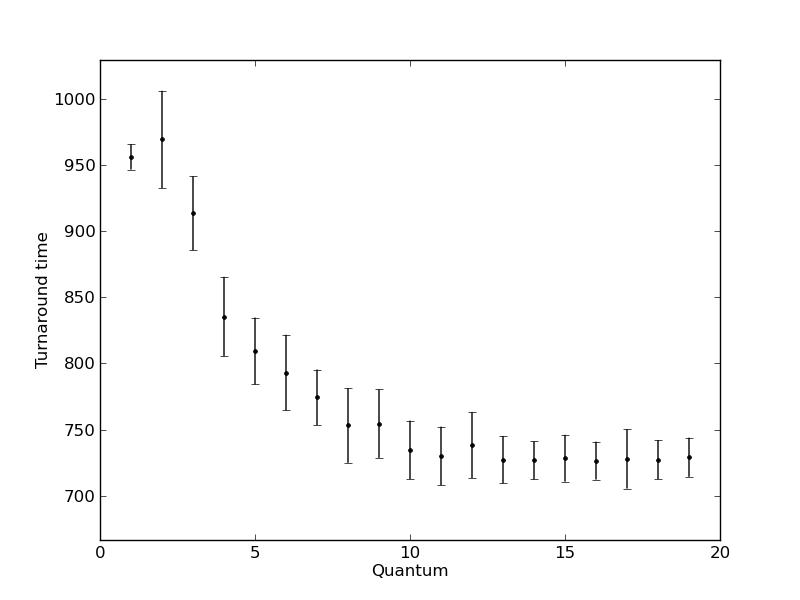
\includegraphics[scale=0.3]{graficos/cores_2_ta.jpg}
		  \caption{Gráfico de Turnaround time en función del quantum con 2 cores para lote de tareas $taskBatch$}
		  \label{fig:contra1}
	\end{center}
\end{figure}

\begin{figure}[H]
	\begin{center}
		  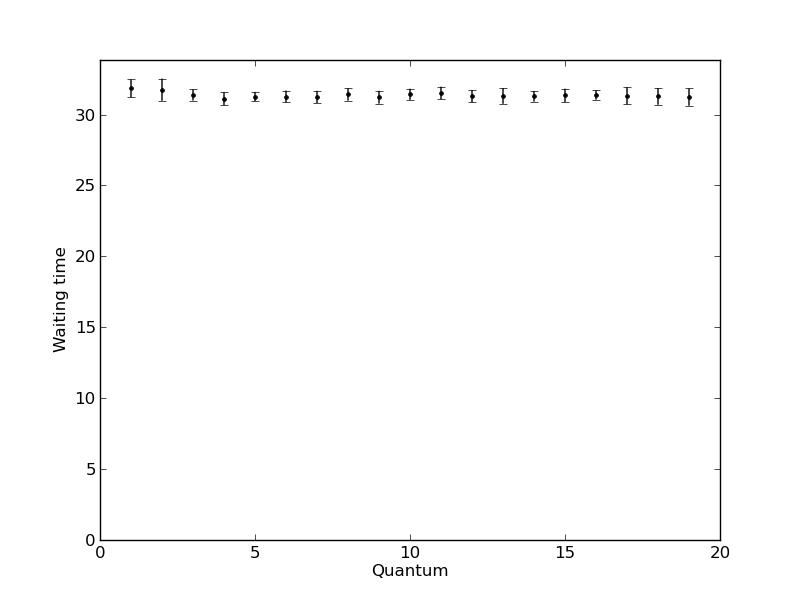
\includegraphics[scale=0.3]{graficos/cores_3_wt.jpg}
		  \caption{Gráfico de Waiting time en función del quantum con 3 cores para lote de tareas $taskBatch$}
		  \label{fig:contra1}
	\end{center}
\end{figure}

\begin{figure}[H]
	\begin{center}
		  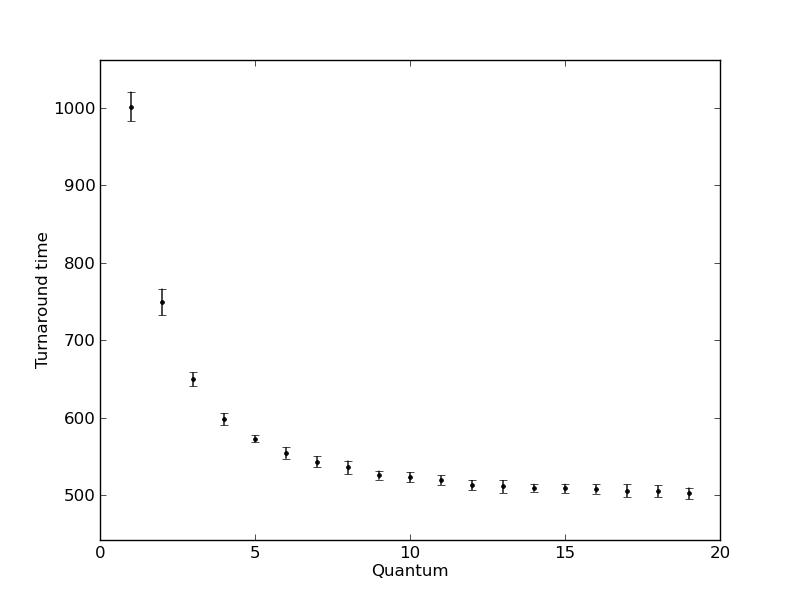
\includegraphics[scale=0.3]{graficos/cores_3_ta.jpg}
		  \caption{Gráfico de Turnaround time en función del quantum con 3 cores para lote de tareas $taskBatch$}
		  \label{fig:contra1}
	\end{center}
\end{figure}

\begin{figure}[H]
	\begin{center}
		  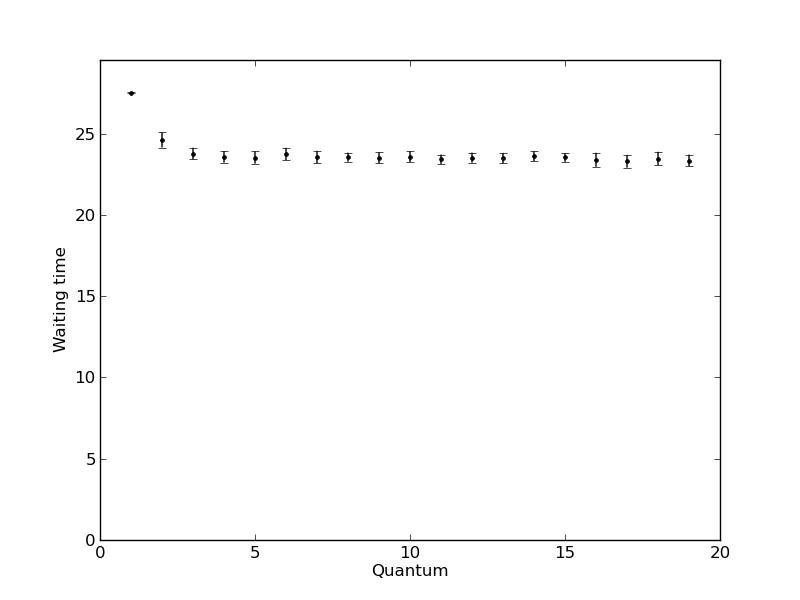
\includegraphics[scale=0.3]{graficos/cores_4_wt.jpg}
		  \caption{Gráfico de Waiting time en función del quantum con 4 cores para lote de tareas $taskBatch$}
		  \label{fig:contra1}
	\end{center}
\end{figure}

\begin{figure}[H]
	\begin{center}
		  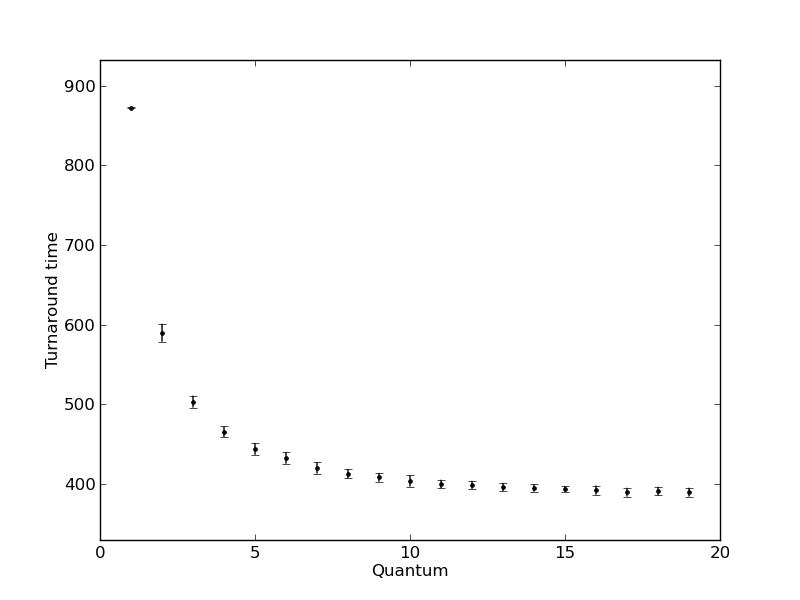
\includegraphics[scale=0.3]{graficos/cores_4_ta.jpg}
		  \caption{Gráfico de Turnaround time en función del quantum con 4 cores para lote de tareas $taskBatch$}
		  \label{fig:contra1}
	\end{center}
\end{figure}

Teniendo en cuenta los gráficos 8, 10 y 12 podemos observar que los valores de waiting time obtenidos para cada quantum no difieren demasiado. Esto no ocurre para los demás graficos en donde el turnaround time comienza a estabilizarse a partir de un quantum igual a 7. Es por esta razón que nos pareció apropiado determinar un quantum óptimo de 7 ticks para el lote de tareas $TaskBatch$ presentado.

